\documentclass[a4paper]{article}

\setlength{\oddsidemargin}{-1in}
\addtolength{\oddsidemargin}{0.05 \paperwidth}
\setlength{\evensidemargin}{-1in}
\addtolength{\evensidemargin}{0.05 \paperwidth}
\setlength{\textwidth}{0.9 \paperwidth}

\setlength{\topmargin}{-0.75in}
\addtolength{\topmargin}{0.05 \paperheight}
\setlength{\textheight}{\paperheight}
\setlength{\headheight}{0in}
\setlength{\headsep}{0in}
\setlength{\footskip}{0in}

\setlength{\parskip}{0.3cm}
\setlength{\parindent}{0pt}
	
\usepackage[T1]{fontenc}
\usepackage[utf8]{inputenc}
\usepackage[german]{babel}
\usepackage{eurosym}

\usepackage[default,scale=1.5]{opensans}
\usepackage[scaled=1.4]{beramono}
\linespread{1.7}

\usepackage{url}
\usepackage{graphicx}

\usepackage{booktabs}


\usepackage{color}
\definecolor{freifunkpink}{RGB}{215,0,73}
\definecolor{freifunkyellow}{RGB}{255,191,0}
\definecolor{lightgrey}{RGB}{220,220,220}

\usepackage{enumitem}
\setlist[itemize]{leftmargin=*}

\begin{document}
\thispagestyle{empty}
 
\begin{center}
\Huge \textit{\textbf{\textcolor{freifunkpink}{Internet für Flüchtlinge}}} \\
\vspace{0.6cm}
\large Bitte teilen sie Ihren Internetzugang mit anderen Menschen
\normalsize

\vspace{2.5cm}
\end{center}

Lieber Nachbar
\vspace{0.5cm}

Freifunk Darmstadt ist eine lokales Projekt mit dem Ziel, in Darmstadt und Umgebung ein offenes und kostenloses WLAN-Netzwerk aufzubauen. Wir stellen Technik bereit, mit der jeder seinen Internetzugang mit anderen teilen kann, ohne Abmahnungen oder andere Konsequenzen zu riskieren.

Die Flüchtlinge, die seit kurzem Ihre Nachbarn sind, benötigen einen Internetzugang, um Kontakt mit ihrer Familie und ihrer alten Heimat zu halten. Die meisten haben bereits ein Smartphone oder ein anderes internetfähiges Gerät, sie können sich aber die vergleichsweise teuren Datentarife der Mobilfunkanbieter nicht leisten.

Zur Zeit unterstützen schon etwa 170 Menschen in Darmstadt und Umgebung Freifunk und teilen ihren Internetzugang. In der Nähe der Flüchtlingslager gibt es zur Zeit noch nicht genug Zugangspunkte um eine vollständige Versorgung zu gewährleisten.

Jeder kann selbst einen Router für Freifunk installieren. Eine Liste von geeigneten Geräten haben wir auf der Rückseite zusammen gestellt. Wenn es zu Problemen kommt, helfen wir gerne.
Wenn ihr euch mit der technischen Seite nicht beschäftigen wollt, könnt ihr auch von uns vorbereitete Geräte bekommen.

\vspace{1cm}

\begin{center}

\includegraphics[width=\textwidth]{logo}
\end{center}

\newpage

\thispagestyle{empty}

\textbf{Unterstützte Geräte}

\begin{center}
\begin{tabular}{ccc} \toprule
	Modell & Preis & gleichzeitige Benutzer\\ \midrule
	TP-Link TL-WR841 (N oder ND) & ca. \EUR{16} & bis zu 15 \\
	TP-Link TL-WR842 (N oder ND) & ca. \EUR{30} & bis zu 30 \\
	TP-Link TL-WR1043 (N oder ND) & ca. \EUR{40} & bis zu 40 \\
	TP-Link TL-WR1043 (N oder ND) & ca. \EUR{45} & bis zu 60 \\
	\bottomrule
\end{tabular}
\end{center}

Die meisten Geräte sind online bei z. B. Amazon oder in Darmstadt bei Zimmermann Elektronic  (Kreuzung Rhein-/Neckerstraße) oder Saturn (Fussgängerzone Innenstadt oder Loop5) erhältlich.

\begin{center}
\vspace{.5cm}
\hspace*{-0.05 \paperwidth}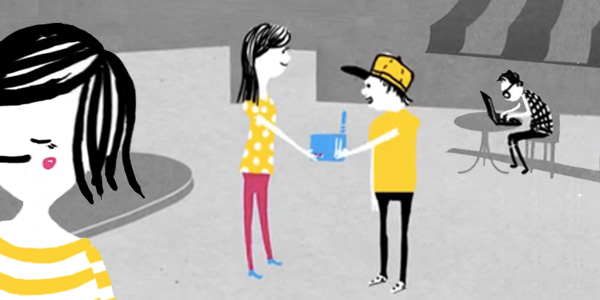
\includegraphics[width=\paperwidth]{community}
\vspace{.5cm}
\end{center}

Witere Informationen über uns findet ihr auf \textbf{http://darmstadt.freifunk.net}, für Fragen stehen wir auch unter \textbf{info@darmstadt.freifunk.net} zur Verfügung.

Gerne könnt ihr auch zu unseren \textbf{wöchentlichen Treffen} jeden Montag um 19:00 Uhr in der Willhelm-Leuschner-Straße 36 (Im Hinterhof) in Darmstadt kommen.


\end{document}
